%% knit("diamond_neph_lfreq_model.Rnw")

\documentclass[12pt]{article}\usepackage[]{graphicx}\usepackage[]{color}
%% maxwidth is the original width if it is less than linewidth
%% otherwise use linewidth (to make sure the graphics do not exceed the margin)
\makeatletter
\def\maxwidth{ %
  \ifdim\Gin@nat@width>\linewidth
    \linewidth
  \else
    \Gin@nat@width
  \fi
}
\makeatother

\definecolor{fgcolor}{rgb}{0.345, 0.345, 0.345}
\newcommand{\hlnum}[1]{\textcolor[rgb]{0.686,0.059,0.569}{#1}}%
\newcommand{\hlstr}[1]{\textcolor[rgb]{0.192,0.494,0.8}{#1}}%
\newcommand{\hlcom}[1]{\textcolor[rgb]{0.678,0.584,0.686}{\textit{#1}}}%
\newcommand{\hlopt}[1]{\textcolor[rgb]{0,0,0}{#1}}%
\newcommand{\hlstd}[1]{\textcolor[rgb]{0.345,0.345,0.345}{#1}}%
\newcommand{\hlkwa}[1]{\textcolor[rgb]{0.161,0.373,0.58}{\textbf{#1}}}%
\newcommand{\hlkwb}[1]{\textcolor[rgb]{0.69,0.353,0.396}{#1}}%
\newcommand{\hlkwc}[1]{\textcolor[rgb]{0.333,0.667,0.333}{#1}}%
\newcommand{\hlkwd}[1]{\textcolor[rgb]{0.737,0.353,0.396}{\textbf{#1}}}%

\usepackage{framed}
\makeatletter
\newenvironment{kframe}{%
 \def\at@end@of@kframe{}%
 \ifinner\ifhmode%
  \def\at@end@of@kframe{\end{minipage}}%
  \begin{minipage}{\columnwidth}%
 \fi\fi%
 \def\FrameCommand##1{\hskip\@totalleftmargin \hskip-\fboxsep
 \colorbox{shadecolor}{##1}\hskip-\fboxsep
     % There is no \\@totalrightmargin, so:
     \hskip-\linewidth \hskip-\@totalleftmargin \hskip\columnwidth}%
 \MakeFramed {\advance\hsize-\width
   \@totalleftmargin\z@ \linewidth\hsize
   \@setminipage}}%
 {\par\unskip\endMakeFramed%
 \at@end@of@kframe}
\makeatother

\definecolor{shadecolor}{rgb}{.97, .97, .97}
\definecolor{messagecolor}{rgb}{0, 0, 0}
\definecolor{warningcolor}{rgb}{1, 0, 1}
\definecolor{errorcolor}{rgb}{1, 0, 0}
\newenvironment{knitrout}{}{} % an empty environment to be redefined in TeX

\usepackage{alltt}
\usepackage{times}
\usepackage{hyperref}
\hypersetup{pdfpagemode=UseNone} % don't show bookmarks on initial view
\hypersetup{colorlinks, urlcolor={blue}}

% revise margins
\setlength{\headheight}{0.0in}
\setlength{\topmargin}{0.0in}
\setlength{\headsep}{0.0in}
\setlength{\textheight}{8.65in}
\setlength{\footskip}{0.35in}
\setlength{\oddsidemargin}{0.0in}
\setlength{\evensidemargin}{0.0in}
\setlength{\textwidth}{6.5in}

\setlength{\parskip}{6pt}
\setlength{\parindent}{0pt}

\title{A model for changes in length frequencies}
\author{}
\date{}
\IfFileExists{upquote.sty}{\usepackage{upquote}}{}
\begin{document}



\maketitle

\section{Data}
Read in length data and modify some column names and variable labels for use below.

\begin{knitrout}\footnotesize
\definecolor{shadecolor}{rgb}{0.969, 0.969, 0.969}\color{fgcolor}\begin{kframe}
\begin{alltt}
\hlkwd{library}\hlstd{(gdata)}

\hlkwd{setwd}\hlstd{(}\hlstr{"../data"}\hlstd{)}

\hlstd{neph.dat} \hlkwb{<-} \hlkwd{read.xls}\hlstd{(}\hlstr{"Celtic Warrior Diamond mesh July 2014 Celtic Sea.xls"}\hlstd{,}
    \hlkwc{sheet} \hlstd{=} \hlstr{"Nephrops Lengths"}\hlstd{,} \hlkwc{stringsAsFactors} \hlstd{=} \hlnum{FALSE}\hlstd{)}

\hlcom{## Show the first 2 rows}
\hlkwd{head}\hlstd{(neph.dat,} \hlnum{2}\hlstd{)}
\end{alltt}
\begin{verbatim}
##           Vessel       DATE HAUL COMPARTMENT Mesh.Size  SPECIES
## 1 Celtic Warrior 2014-07-19    1     Control      70mm Nephrops
## 2 Celtic Warrior 2014-07-19    1     Control      70mm Nephrops
##   Carapace.Length..mm.. COUNT SUBSRATIO
## 1                    16     1         1
## 2                    17    11         1
\end{verbatim}
\begin{alltt}
\hlcom{## Change the carapace length name}
\hlkwd{names}\hlstd{(neph.dat)[}\hlkwd{names}\hlstd{(neph.dat)} \hlopt{==} \hlstr{"Carapace.Length..mm.."}\hlstd{]} \hlkwb{<-} \hlstr{"Carapace.Length"}

\hlcom{## Make the 'HAUL' variable character}
\hlstd{neph.dat}\hlopt{$}\hlstd{HAUL} \hlkwb{<-} \hlkwd{paste}\hlstd{(}\hlstr{"H"}\hlstd{, neph.dat}\hlopt{$}\hlstd{HAUL,} \hlkwc{sep} \hlstd{=} \hlstr{""}\hlstd{)}
\end{alltt}
\end{kframe}
\end{knitrout}
%% 
Make one row per length measurement assuming, for example, that a sub-sampling ratio of 0.1 corresponds to 10\% of the catch sampled (CHECK).

\begin{knitrout}\footnotesize
\definecolor{shadecolor}{rgb}{0.969, 0.969, 0.969}\color{fgcolor}\begin{kframe}
\begin{alltt}
\hlcom{## get a row per length measurement (raise them also)}
\hlstd{n} \hlkwb{<-} \hlkwd{nrow}\hlstd{(neph.dat)}

\hlstd{neph.dat2} \hlkwb{<-} \hlstd{neph.dat[}\hlkwd{rep}\hlstd{(}\hlnum{1}\hlopt{:}\hlstd{n,} \hlkwc{times} \hlstd{=} \hlkwd{round}\hlstd{(neph.dat}\hlopt{$}\hlstd{COUNT}\hlopt{/}\hlstd{neph.dat}\hlopt{$}\hlstd{SUBSRATIO,}
    \hlnum{0}\hlstd{)), ]}
\end{alltt}
\end{kframe}
\end{knitrout}
%% 
Read in the haul weights
\begin{knitrout}\footnotesize
\definecolor{shadecolor}{rgb}{0.969, 0.969, 0.969}\color{fgcolor}\begin{kframe}
\begin{alltt}
\hlkwd{setwd}\hlstd{(}\hlstr{"../data"}\hlstd{)}

\hlstd{weight.dat} \hlkwb{<-} \hlkwd{read.xls}\hlstd{(}\hlstr{"Celtic Warrior Diamond mesh July 2014 Celtic Sea.xls"}\hlstd{,}
    \hlkwc{sheet} \hlstd{=} \hlstr{"Weights"}\hlstd{,} \hlkwc{stringsAsFactors} \hlstd{=} \hlnum{FALSE}\hlstd{)}

\hlcom{## Show the first 2 rows}
\hlkwd{head}\hlstd{(weight.dat,} \hlnum{2}\hlstd{)}
\end{alltt}
\begin{verbatim}
##         Date Haul.. Compartment Mesh.Size Species Total.weight..kg.
## 1 2014-07-19      1       TEST1      90mm    Bulk             26.28
## 2 2014-07-19      1       TEST1      90mm Haddock              0.38
##   Sbsample.weight..kg.
## 1                     
## 2
\end{verbatim}
\begin{alltt}
\hlcom{## create a new 'HAUL' variable for the merge}
\hlstd{weight.dat}\hlopt{$}\hlstd{HAUL} \hlkwb{<-} \hlkwd{paste}\hlstd{(}\hlstr{"H"}\hlstd{, weight.dat}\hlopt{$}\hlstd{Haul..,} \hlkwc{sep} \hlstd{=} \hlstr{""}\hlstd{)}

\hlcom{## re-name total weight column}
\hlkwd{names}\hlstd{(weight.dat)[}\hlkwd{names}\hlstd{(weight.dat)} \hlopt{==} \hlstr{"Total.weight..kg."}\hlstd{]} \hlkwb{<-} \hlstr{"Total.Weight"}
\end{alltt}
\end{kframe}
\end{knitrout}

Merge the bulk weights with the length data
\begin{knitrout}\footnotesize
\definecolor{shadecolor}{rgb}{0.969, 0.969, 0.969}\color{fgcolor}\begin{kframe}
\begin{alltt}
\hlstd{neph.dat3} \hlkwb{<-} \hlkwd{merge}\hlstd{(neph.dat2,}
                   \hlkwd{subset}\hlstd{(weight.dat, Species} \hlopt{==} \hlstr{"Bulk"}\hlstd{)[,} \hlkwd{c}\hlstd{(}\hlstr{"Mesh.Size"}\hlstd{,} \hlstr{"HAUL"}\hlstd{,}
                                        \hlstr{"Total.Weight"}\hlstd{)],}
                   \hlkwc{by} \hlstd{=} \hlkwd{c}\hlstd{(}\hlstr{"Mesh.Size"}\hlstd{,} \hlstr{"HAUL"}\hlstd{))}

\hlcom{## subset the data by mesh size}
\hlstd{neph.70mm} \hlkwb{<-} \hlkwd{subset}\hlstd{(neph.dat3, Mesh.Size} \hlopt{==} \hlstr{"70mm"}\hlstd{)}
\hlstd{neph.80mm} \hlkwb{<-} \hlkwd{subset}\hlstd{(neph.dat3, Mesh.Size} \hlopt{==} \hlstr{"80mm"}\hlstd{)}
\hlstd{neph.90mm} \hlkwb{<-} \hlkwd{subset}\hlstd{(neph.dat3, Mesh.Size} \hlopt{==} \hlstr{"90mm"}\hlstd{)}
\hlstd{neph.100mm} \hlkwb{<-} \hlkwd{subset}\hlstd{(neph.dat3, Mesh.Size} \hlopt{==} \hlstr{"100mm"}\hlstd{)}

\hlcom{## convert HAUL to factor}
\hlcom{## with levels depending on the haul weight}
\hlstd{neph.70mm}\hlopt{$}\hlstd{HAUL} \hlkwb{<-} \hlkwd{factor}\hlstd{(neph.70mm}\hlopt{$}\hlstd{HAUL,} \hlkwc{levels} \hlstd{=}
                         \hlkwd{unique}\hlstd{(neph.70mm}\hlopt{$}\hlstd{HAUL[}\hlkwd{order}\hlstd{(neph.70mm}\hlopt{$}\hlstd{Total.Weight)]))}
\hlstd{neph.80mm}\hlopt{$}\hlstd{HAUL} \hlkwb{<-} \hlkwd{factor}\hlstd{(neph.80mm}\hlopt{$}\hlstd{HAUL,} \hlkwc{levels} \hlstd{=}
                         \hlkwd{unique}\hlstd{(neph.80mm}\hlopt{$}\hlstd{HAUL[}\hlkwd{order}\hlstd{(neph.80mm}\hlopt{$}\hlstd{Total.Weight)]))}
\hlstd{neph.90mm}\hlopt{$}\hlstd{HAUL} \hlkwb{<-} \hlkwd{factor}\hlstd{(neph.90mm}\hlopt{$}\hlstd{HAUL,} \hlkwc{levels} \hlstd{=}
                         \hlkwd{unique}\hlstd{(neph.90mm}\hlopt{$}\hlstd{HAUL[}\hlkwd{order}\hlstd{(neph.90mm}\hlopt{$}\hlstd{Total.Weight)]))}
\hlstd{neph.100mm}\hlopt{$}\hlstd{HAUL} \hlkwb{<-} \hlkwd{factor}\hlstd{(neph.100mm}\hlopt{$}\hlstd{HAUL,} \hlkwc{levels} \hlstd{=}
                          \hlkwd{unique}\hlstd{(neph.100mm}\hlopt{$}\hlstd{HAUL[}\hlkwd{order}\hlstd{(neph.100mm}\hlopt{$}\hlstd{Total.Weight)]))}
\end{alltt}
\end{kframe}
\end{knitrout}


%% 
Produce a summary plot of the data by length, haul and catch weight.
%%
\begin{knitrout}\footnotesize
\definecolor{shadecolor}{rgb}{0.969, 0.969, 0.969}\color{fgcolor}\begin{kframe}
\begin{alltt}
\hlkwd{library}\hlstd{(ggplot2)}
\hlkwd{library}\hlstd{(gridExtra)}

\hlcom{## quick function for plot}
\hlstd{plot.lfreq} \hlkwb{<-} \hlkwa{function}\hlstd{(}\hlkwc{data}\hlstd{,} \hlkwc{title.string}\hlstd{)\{}
  \hlstd{p} \hlkwb{<-} \hlkwd{ggplot}\hlstd{(data,} \hlkwd{aes}\hlstd{(}\hlkwc{x} \hlstd{= Carapace.Length,} \hlkwc{group} \hlstd{= HAUL))} \hlopt{+}
    \hlkwd{geom_density}\hlstd{(}\hlkwc{position} \hlstd{=} \hlstr{"stack"}\hlstd{,}
                 \hlkwd{aes}\hlstd{(}\hlkwc{fill} \hlstd{= Total.Weight),}
                 \hlkwc{colour} \hlstd{=} \hlnum{1}\hlstd{,} \hlkwc{lwd} \hlstd{=} \hlnum{0.005}\hlstd{)} \hlopt{+}
                 \hlkwd{xlim}\hlstd{(}\hlnum{10}\hlstd{,} \hlnum{45}\hlstd{)} \hlopt{+}
                 \hlkwd{scale_fill_gradient2}\hlstd{(}\hlkwc{low} \hlstd{=} \hlstr{"white"}\hlstd{,} \hlkwc{high} \hlstd{=} \hlstr{"blue"}\hlstd{,}
                                      \hlkwc{limits} \hlstd{=} \hlkwd{c}\hlstd{(}\hlnum{0}\hlstd{,} \hlkwd{max}\hlstd{(neph.dat3}\hlopt{$}\hlstd{Total.Weight)))} \hlopt{+}
                 \hlkwd{ggtitle}\hlstd{(title.string)} \hlopt{+}
                 \hlkwd{theme}\hlstd{(}\hlkwc{axis.text.x}\hlstd{=}\hlkwd{element_blank}\hlstd{())}
  \hlkwd{return}\hlstd{(p)}
\hlstd{\}}

\hlstd{p70mm} \hlkwb{<-} \hlkwd{plot.lfreq}\hlstd{(neph.70mm,} \hlstr{"70mm"}\hlstd{)}
\hlstd{p80mm} \hlkwb{<-} \hlkwd{plot.lfreq}\hlstd{(neph.80mm,} \hlstr{"80mm"}\hlstd{)}
\hlstd{p90mm} \hlkwb{<-} \hlkwd{plot.lfreq}\hlstd{(neph.90mm,} \hlstr{"90mm"}\hlstd{)}
\hlstd{p100mm} \hlkwb{<-} \hlkwd{plot.lfreq}\hlstd{(neph.100mm,} \hlstr{"100mm"}\hlstd{)}

\hlkwd{grid.arrange}\hlstd{(p70mm, p80mm, p90mm, p100mm,} \hlkwc{ncol} \hlstd{=} \hlnum{1}\hlstd{)}
\end{alltt}
\end{kframe}\begin{figure}

{\centering 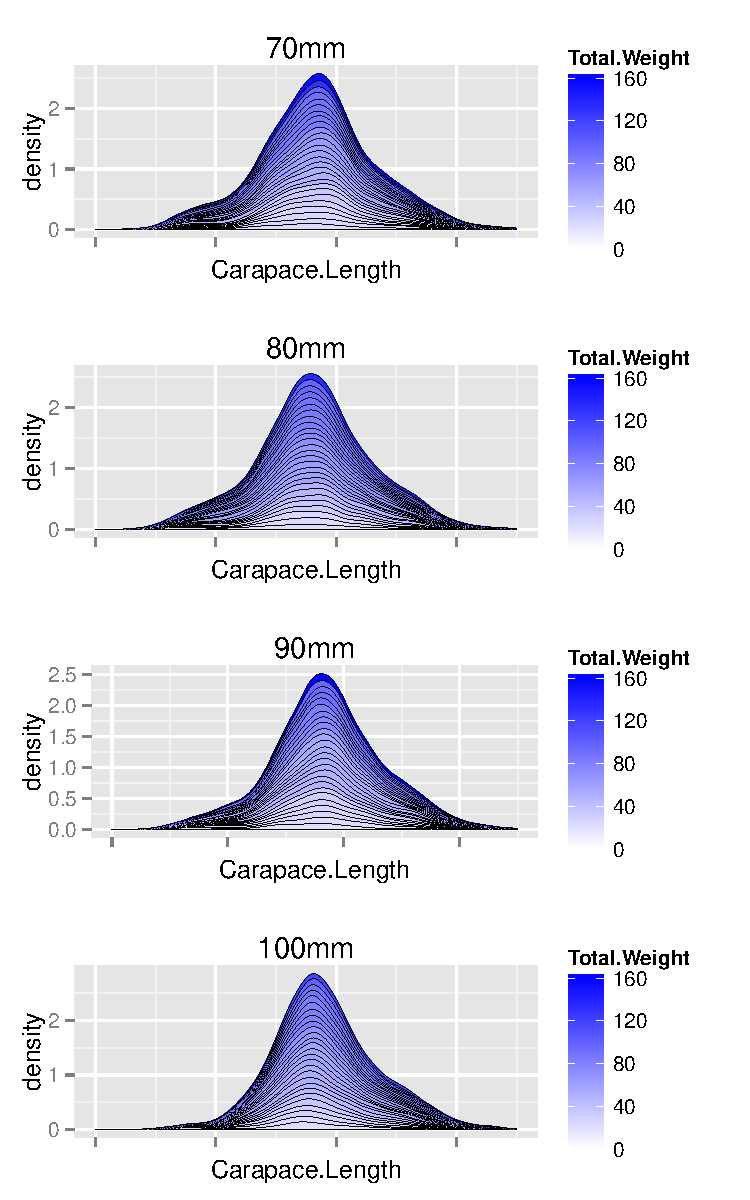
\includegraphics[width=\maxwidth]{figure/unnamed-chunk-6-1} 

}

\caption[Stacked carapace length densities]{Stacked carapace length densities. Each haul is coloured according to the total bulk weight in that haul.}\label{fig:unnamed-chunk-6}
\end{figure}


\end{knitrout}

\end{document}
